\documentclass[12pt]{article}
 
\usepackage[margin=1in]{geometry} 
\usepackage{amsmath,amsthm,amssymb, graphicx, multicol, array}
\usepackage{parskip}
\usepackage{booktabs}
\usepackage{subfigure}

 \usepackage{amsmath}
\usepackage{amsfonts}
\usepackage{amssymb}
\usepackage[version=4]{mhchem}
\usepackage{stmaryrd}
\usepackage[margin=1in]{geometry} 
\usepackage{amsmath,amsthm,amssymb, graphicx, multicol, array}
\usepackage{parskip}
\usepackage{booktabs}

 
\newcommand{\N}{\mathbb{N}}
\newcommand{\Z}{\mathbb{Z}}
 

\begin{document}
 
\title{Problem Set 6}
\author{Nicolas Moreno, Kushal Patel, Olivia Wilkinson \\
ECON: 880}
\maketitle

\section{Exercise 1}
We started with the suggested N, but it had to be increased gradually to N=51. This means that after the reform it takes this long to get to the new steady state where there's no social security.

Below you can find a table with the two steady states compared. These show that in the absence of the pay-as-you-go pension system, households react by increasing savings. Higher savings translate into higher aggregate capital and by complementarity higher labor demand. Under the parameters used in the model, wages increase and the interest rate falls.

\begin{table}[h!]
    \centering
    \caption{Policy experiment results }
    \begin{tabular}{|c|c|c|c|c|c|c|}
    \hline
         & \multicolumn{2}{c|}{Steady States} \\
         \hline 
         & with ss & no ss \\
         \hline
         Capital ($K$) & 3.36 & 4.59  \\
         Labor ($L$) & 0.34 & 0.37 \\
         Wage ($W$)  & 1.46 & 1.59  \\
         Interest Rate ($R$) & 0.02 & 0.01\\
         Pension Benefit ($B$) & 0.23 & 0.00 \\
         \hline 
    \end{tabular}
    \label{tab:policyres}
\end{table}

Given the comparative statics we just discussed, we should expect transition paths for capital and labor that lead to their higher equilibrium levels. However, because capital is a stock, this process would be gradual and it would take time for the economy to build it. In contrast, labor can adjust immediately, since we are assuming no labor market or labor supply frictions. Because agents realize they need to save more after the MIT shock, they should work more from $T=0$. The figures of the simulation transition path verify this analysis.\\

\begin{figure}[hbt!]
    \centering
    \vspace{1cm}
    \subfigure{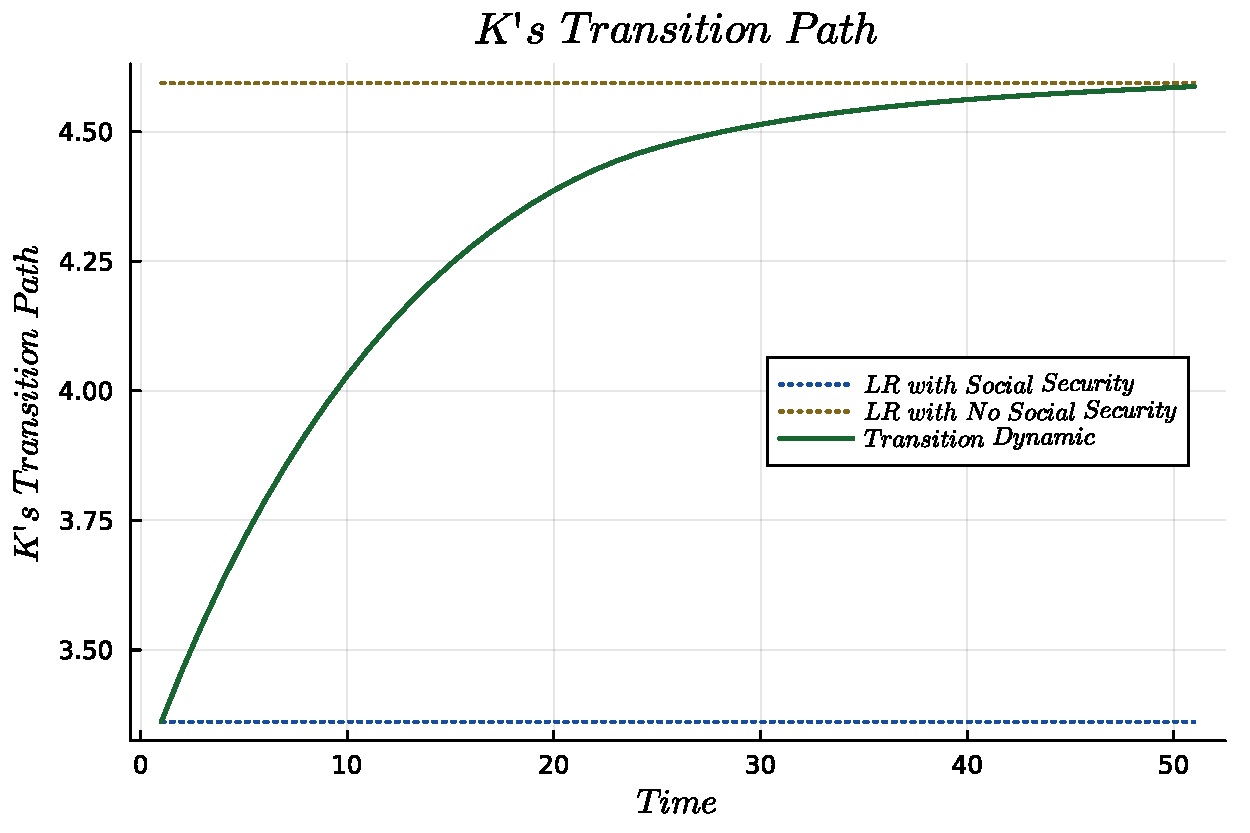
\includegraphics[width=0.435\textwidth]{Computational/ECON 880 Q1/PS6/Figures_Exercise1/K_Transition_Path.pdf}    }
\subfigure{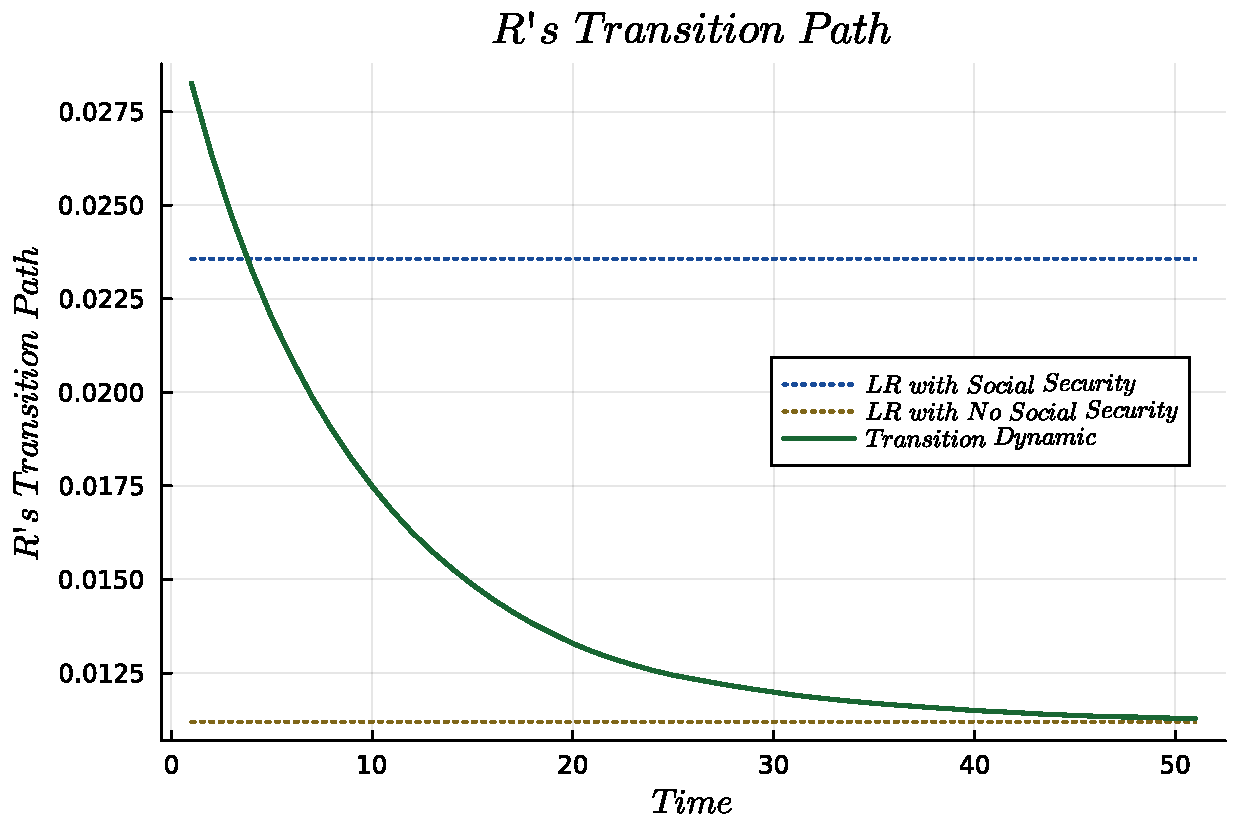
\includegraphics[width=0.435\textwidth]{Computational/ECON 880 Q1/PS6/Figures_Exercise1/R_Transition_Path.pdf}}
\subfigure{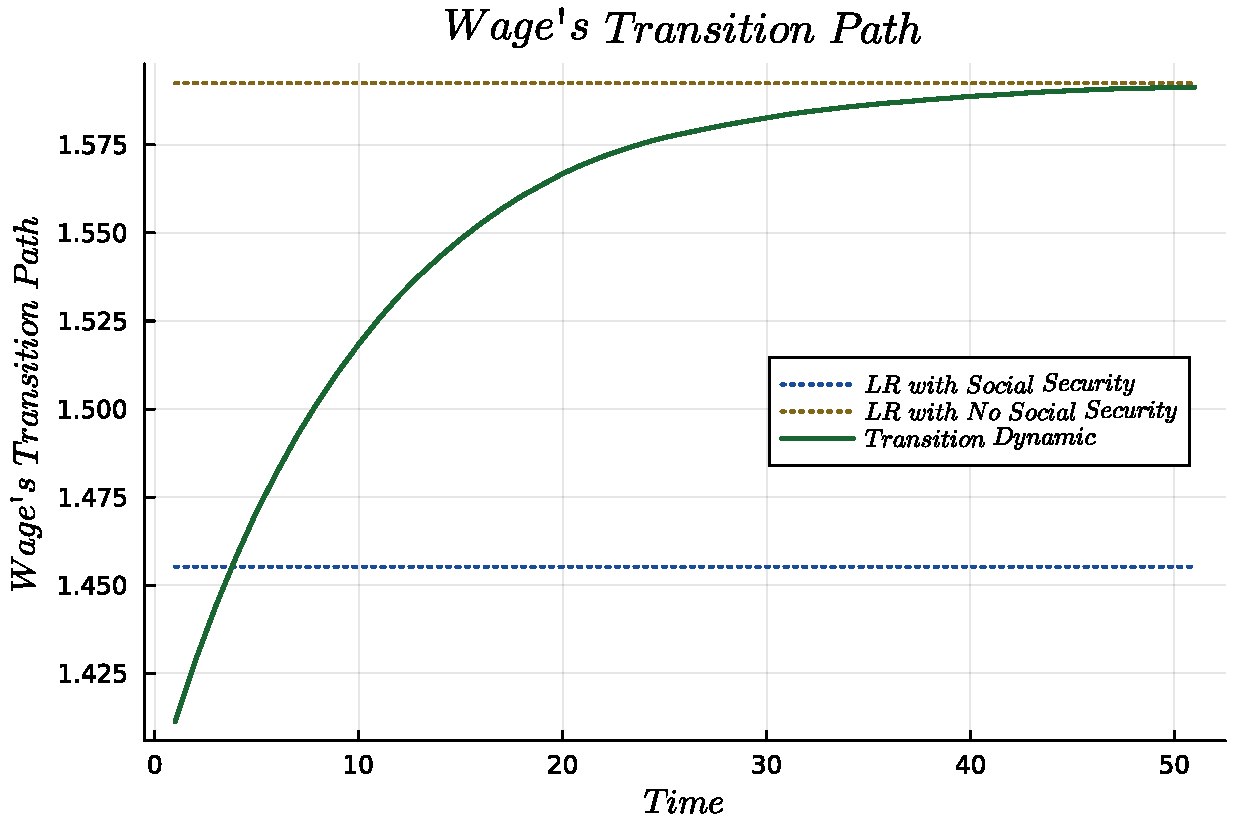
\includegraphics[width=0.435\textwidth]{Computational/ECON 880 Q1/PS6/Figures_Exercise1/W_Transition_Path.pdf}}
\subfigure{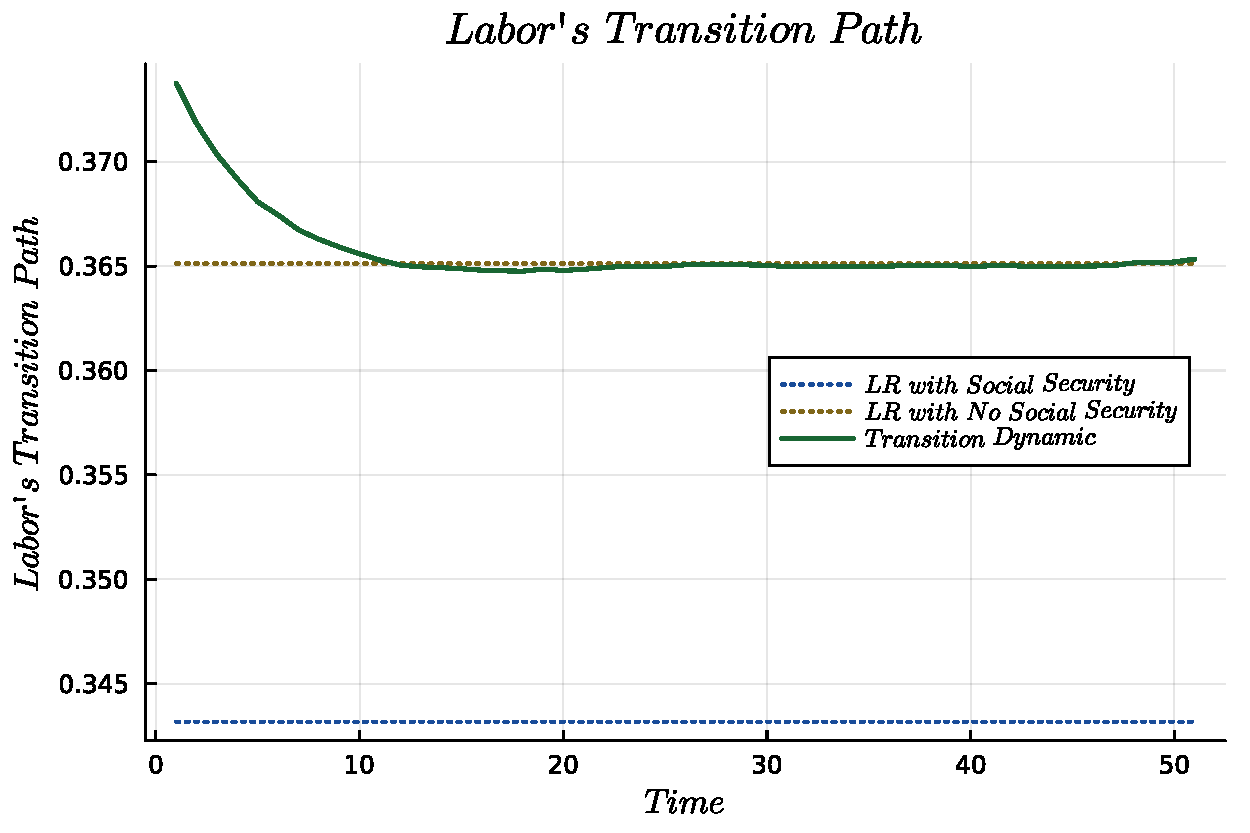
\includegraphics[width=0.435\textwidth]{Computational/ECON 880 Q1/PS6/Figures_Exercise1/L_Transition_Path.pdf} }   
\end{figure}
\newpage

Regarding the welfare impact of the reform, we can see in the graph below the average consumption equivalent variation across generations to get a sense of the popularity of the reform. This figure depicts how the reform's negative impact (Consumption Equivalent Variation is below 1 and falling towards zero) monotonically increases across all working ages. Then there is a discontinuous jump when people reach their retirement age and is near zero for retired people. The reason for this result is that younger people have a greater chance of adjusting to the reform as they have more time to increase working hours and savings to build up a capital buffer to use in old age. Only 9.98\% of the population would voted in favor of the reform.

\begin{figure}[hbt!]
    \centering
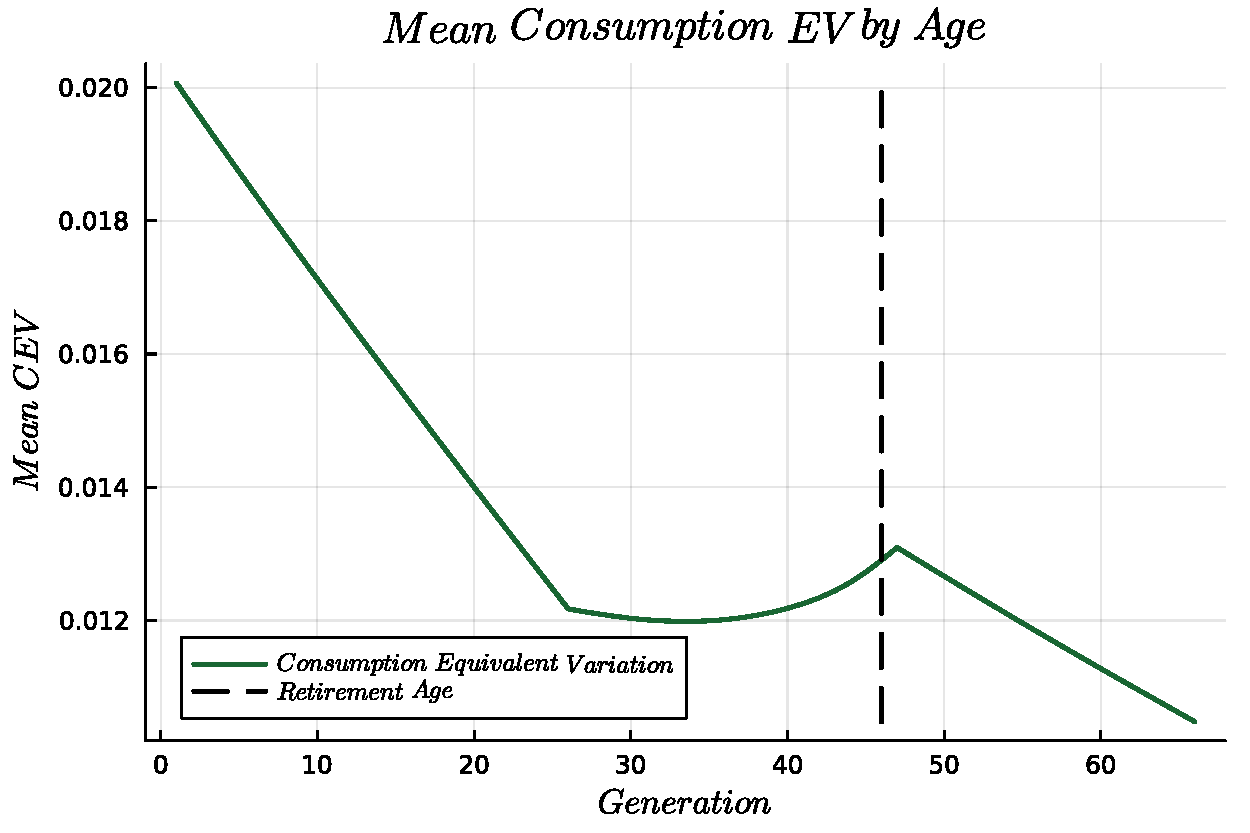
\includegraphics[width=0.5\textwidth]{Computational/ECON 880 Q1/PS6/Figures_Exercise1/CEV1.pdf}
\end{figure}

\newpage

\section{Credible Announcement}
When the government credibly announces that the reform will take place in 21 years, the behavior of the aggregate variables dramatically changes. In particular, aggregate labor no longer overshoots from the start and converges from above to the new steady state as in the first scenario; now, labor modestly increases before the reform is implemented and then overshoots the year after the new rules are active. The future retirees that will retire the year after the reform kicks in want to work significantly more to save for their old age, at that age one would see the peak in working hours. Nonetheless, generations considerably younger or older will want to work less: the former because they can still save enough for old age and the latter because the impact of increased labor on savings monotonically decreases as people are closer to retirement.

\begin{figure}[hbt!]
    \centering
    \vspace{1cm}
    \subfigure{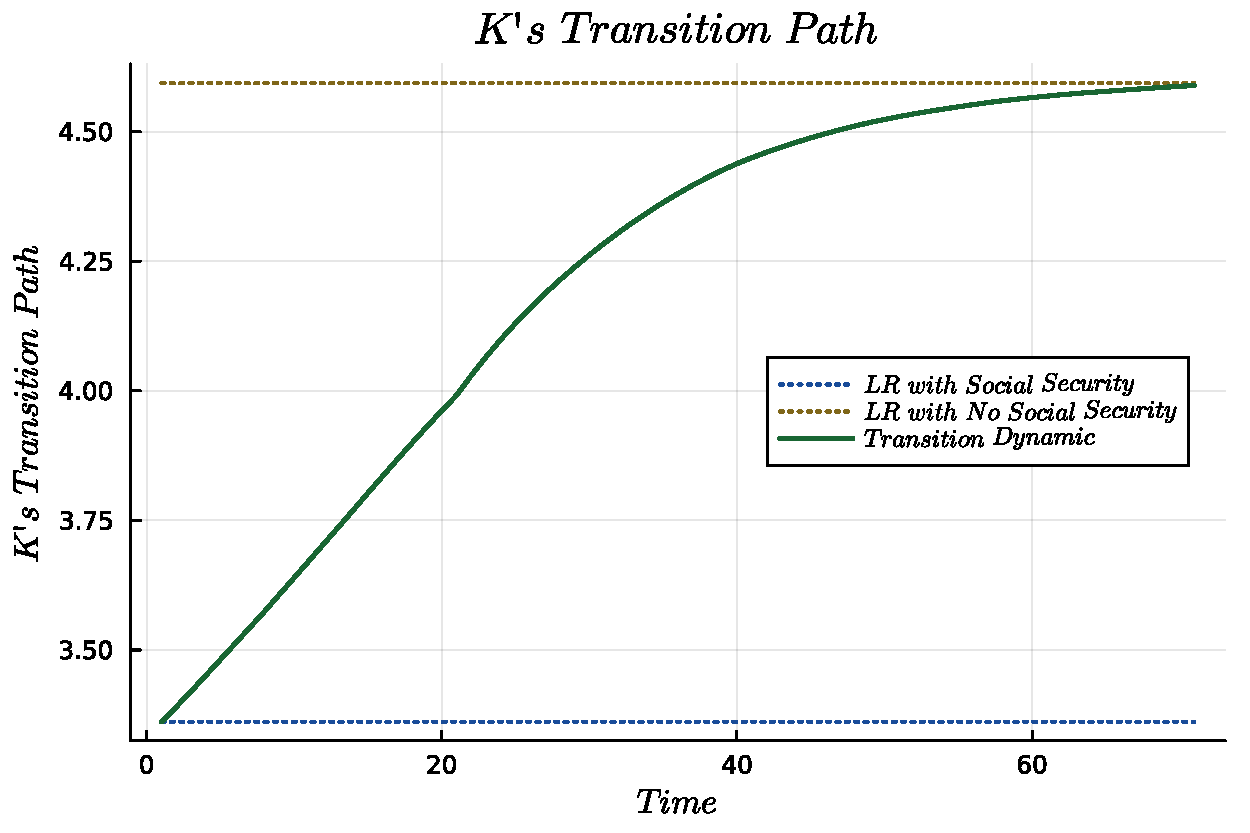
\includegraphics[width=0.435\textwidth]{Computational/ECON 880 Q1/PS6/Figures_Exercise2/K_Transition_Path2.pdf}    }
\subfigure{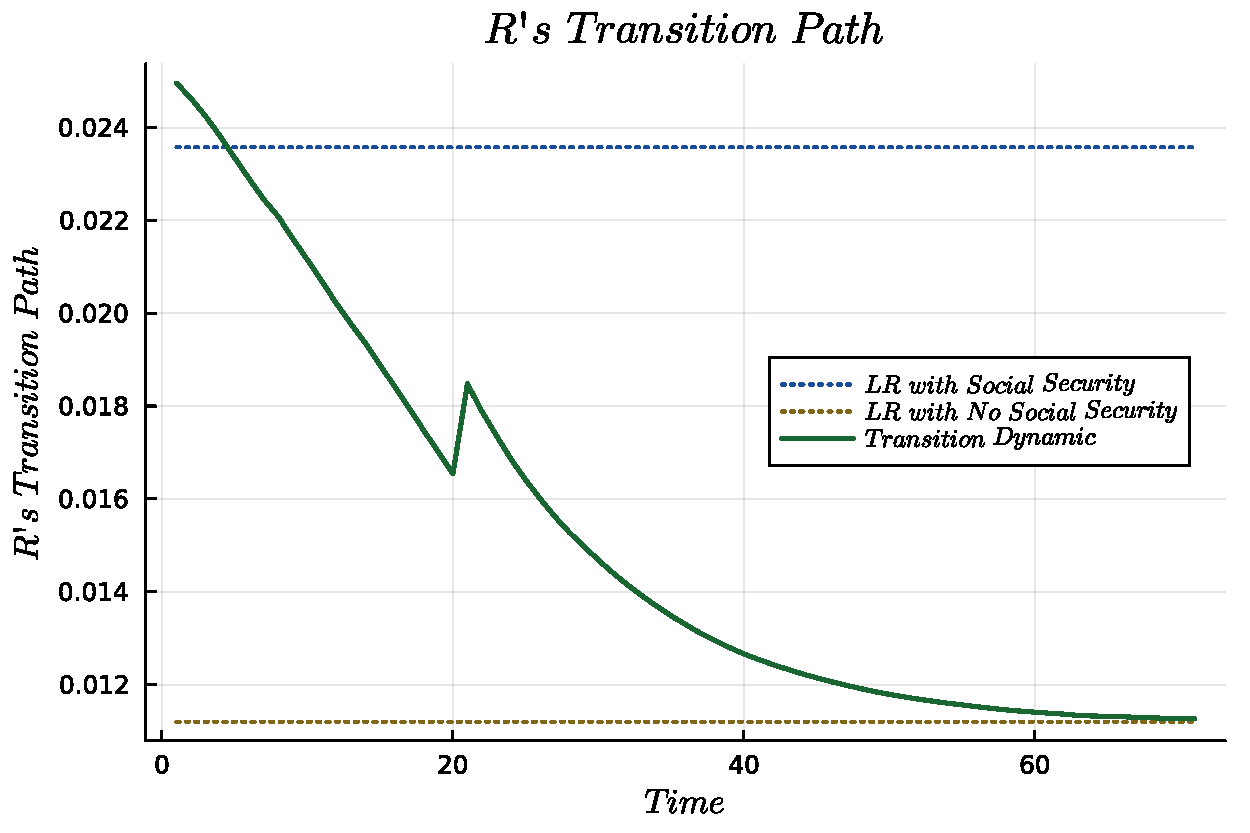
\includegraphics[width=0.435\textwidth]{Computational/ECON 880 Q1/PS6/Figures_Exercise2/R_Transition_Path2.pdf}}
\subfigure{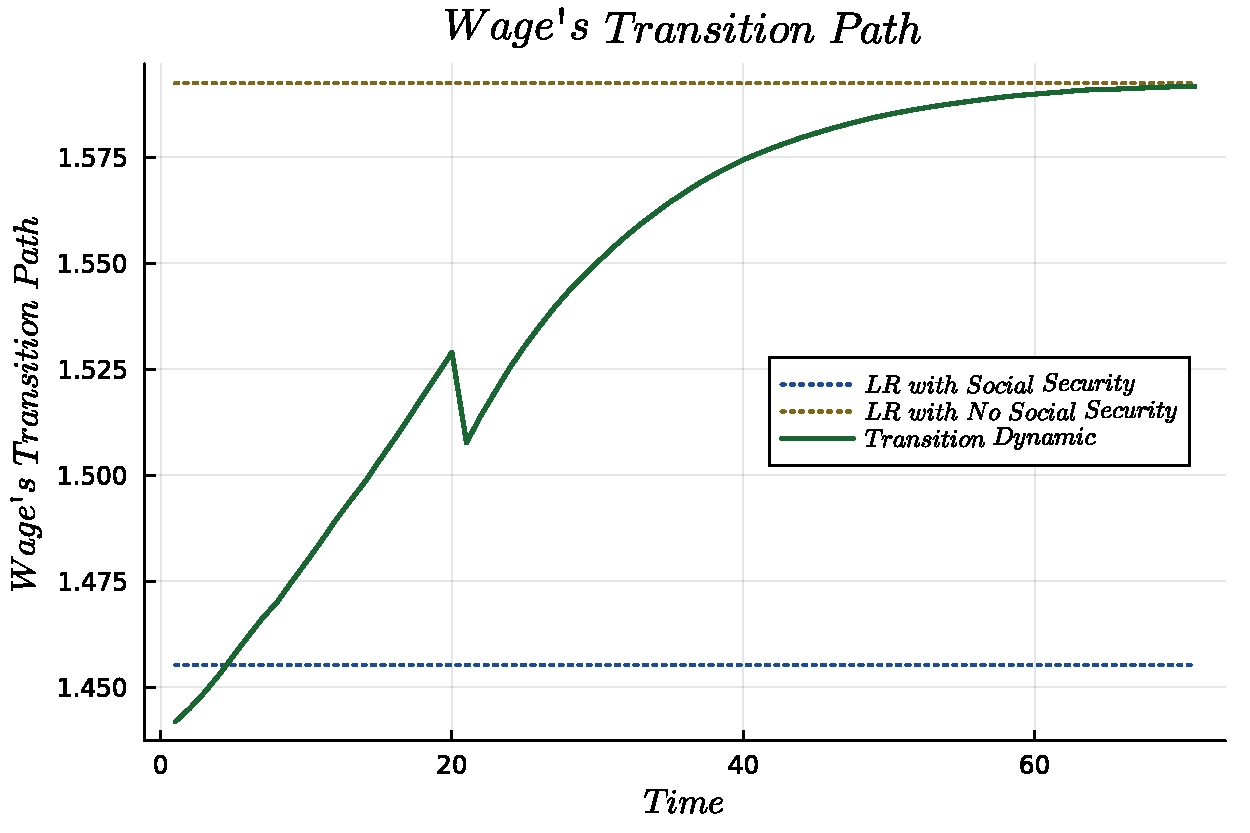
\includegraphics[width=0.435\textwidth]{Computational/ECON 880 Q1/PS6/Figures_Exercise2/W_Transition_Path2.pdf}}
\subfigure{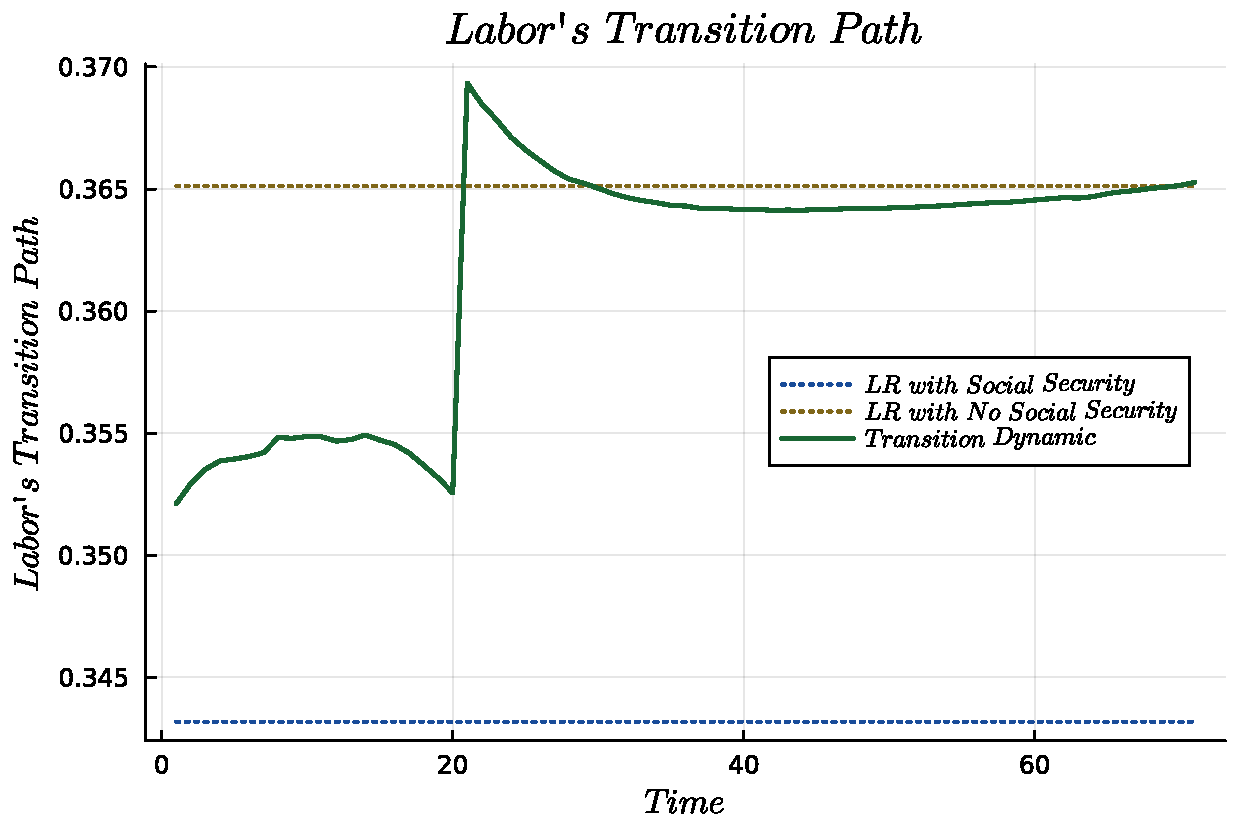
\includegraphics[width=0.435\textwidth]{Computational/ECON 880 Q1/PS6/Figures_Exercise2/L_Transition_Path2.pdf} }   
\end{figure}

The transition dynamics of capital are smoother, again reflecting the fact that this is a stock that can only gradually adjust to shocks. Finally, with the onset of the reform capital income jumps up whereas wages jump down, both being pecuniary externalities that favor those with higher savings and hindering workers. This could potentially increase inequality after the reform is fully implemented. In general, these pecuniary externalities act as indirect mechanisms (general equilibrium mechanisms) that positively affect the retired, as the return on their savings is higher.

\begin{figure}[hbt!]
    \centering
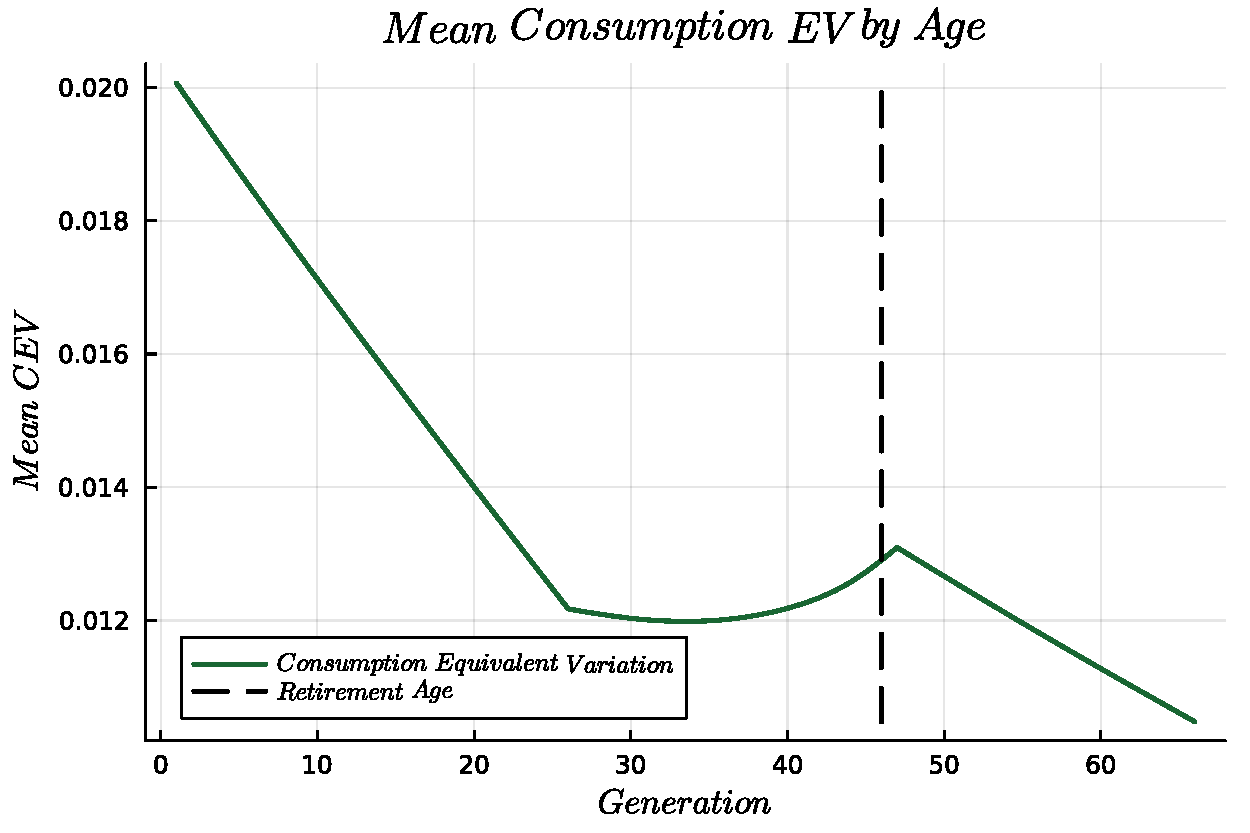
\includegraphics[width=0.5\textwidth]{Computational/ECON 880 Q1/PS6/Figures_Exercise2/CEV2.pdf}
\end{figure}

Clearly, when the reform is designed not to affect directly the retired and older workers, this would mean that the CEV would no longer fall monotonically with generations. Accordingly, the share of voters in favor of the reform increases now to 23.33\%.

\end{document}